\documentclass[12pt]{ximera}
\title{Practice Final Exam}
\begin{document}
\begin{abstract}
Practice for the cumulative final: two-set Venn diagrams and conditional probability,
the subtraction game, counting role assignments with restrictions, saddle points, and
expected value as a decision tool.
\end{abstract}
\maketitle

\section*{Practice Final Exam}

\begin{problem}
Assess whether each of the following claims is true or false.

\begin{prompt}
\textbf{(a)} Claim: the payoff matrix for any two-player zero-sum game has a
\emph{saddle point} (a possible outcome where neither player is motivated to deviate
from their corresponding strategy).

\begin{multipleChoice}
\choice{True}
\choice[correct]{False}
\end{multipleChoice}

\begin{feedback}
False. Plenty of games have no saddle point. For instance,
\[
\begin{array}{c|c|c|}
\phantom{|} & c & d \\\hline
a & 4 & -3 \\\hline
b & -1 & 1 \\\hline
\end{array}
\]
has row minima $-3$ and $-1$ (maximin $-1$) and column maxima $4$ and $1$
(minimax $1$). Since $-1\neq 1$, there is no saddle point --- whichever cell you
land in, one of the two players would rather have chosen differently. Such games have
no stable pure strategy, and both players are better off mixing.
\end{feedback}
\end{prompt}

\begin{prompt}
\textbf{(b)} Claim: the probability of each possible outcome in a two-player simple
game is equal to the product of the probabilities of each player choosing the
strategy associated with that outcome.

\begin{multipleChoice}
\choice[correct]{True}
\choice{False}
\end{multipleChoice}

\begin{feedback}
True, because the two players choose independently --- neither can see the other's
choice before committing. For independent events,
$P(E\cap F)=P(E)\cdot P(F)$, so the probability of a given cell is the product of the
corresponding row and column probabilities.
\end{feedback}
\end{prompt}
\end{problem}

\begin{problem}
In a survey of $200$ people, $115$ said they would accept calling a hotdog on a bun a
``sandwich'' (S), $95$ said they would accept calling it a ``taco'' (T), and $55$ said
they would accept calling it either.

\begin{prompt}
\textbf{(a)} Fill in all four regions of the Venn diagram.

\begin{center}
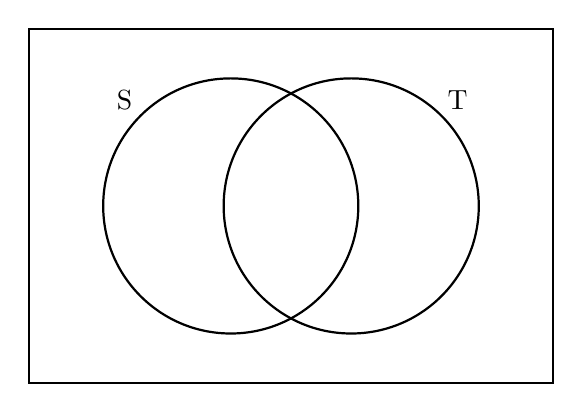
\begin{tikzpicture}[scale=0.9]
  \draw[thick] (-0.85,0) circle (1.8) node at (-2.35,1.5) {S};
  \draw[thick] (0.85,0) circle (1.8) node at (2.35,1.5) {T};
  \draw[thick] (-3.7,-2.5) rectangle (3.7,2.5);
\end{tikzpicture}
\end{center}

S only: $\answer{60}$ \qquad
Both: $\answer{55}$ \qquad
T only: $\answer{40}$ \qquad
Neither: $\answer{45}$

\begin{feedback}
The overlap is $55$, so
\[
\text{S only} = 115-55 = 60, \qquad \text{T only} = 95-55 = 40.
\]
Those three regions total $60+55+40=155$, leaving $200-155=45$ people who would
accept neither name.
\end{feedback}
\end{prompt}

\begin{prompt}
\textbf{(b)} What is the (conditional) probability that someone who would accept
calling a hotdog on a bun a ``taco'' would NOT accept calling it a ``sandwich''?

Give your answer as a fraction in lowest terms: $\answer{8/19}$

\begin{hint}
Restrict to the $95$ people in the T circle. How many of them lie outside S?
\end{hint}

\begin{feedback}
Of the $95$ people who would accept ``taco'', $40$ are in the ``T only'' region, so
\[
P\!\left(\olsi{S}\mid T\right)=\frac{40}{95}=\frac{8}{19}\approx 0.421.
\]
\end{feedback}
\end{prompt}
\end{problem}

\begin{problem}
Alice and Bob are playing a variation of the Subtraction Game with the following
rules:
\begin{itemize}
\item start with $13$ stones in the pile;
\item on each turn, a player can take $1$, $2$, $3$, or $4$ stones;
\item the winner is the player who takes the final stone.
\end{itemize}

\begin{prompt}
If Alice goes first, which player has a winning strategy?

\begin{multipleChoice}
\choice[correct]{Alice, the first player}
\choice{Bob, the second player}
\choice{Neither --- it depends on how Bob plays}
\end{multipleChoice}

How many stones should Alice take on her first turn? $\answer{3}$

\begin{hint}
When a player may take $1$ through $m$ stones, the losing positions are the multiples
of $m+1$. Here $m=4$.
\end{hint}

\begin{feedback}
With moves of $1$ to $4$ stones, the losing positions are the multiples of $5$: from a
pile of $5$, any move leaves between $1$ and $4$, which your opponent simply takes to
win.

Since $13 = 5\cdot 2 + 3$ is not a multiple of $5$, Alice wins. She takes $3$ stones,
leaving $10$. Thereafter she answers each of Bob's moves so that the pair of moves
removes exactly $5$ stones --- if Bob takes $k$, she takes $5-k$. Bob then faces
$10$, then $5$, then $0$, so Alice takes the last stone.

Compare this with the version on the Final Exam, where moves of $1$ to $3$ made the
multiples of $4$ the losing positions.
\end{feedback}
\end{prompt}
\end{problem}

\begin{problem}
A theatre director is casting actors for Hadestown and needs to assign the roles of
Hades, Persephone, Eurydice, and Orpheus.

\begin{prompt}
\textbf{(a)} If \emph{ten} actors audition (and any of them can be cast for any of
the roles), how many different ways can these four roles be assigned?

$\answer{5040}$

\begin{hint}
The four roles are distinct, and one actor cannot play two roles.
\end{hint}

\begin{feedback}
This is a permutation, since the roles are distinguishable:
\[ P(10,4)=10\cdot 9\cdot 8\cdot 7 = 5040. \]
\end{feedback}
\end{prompt}

\begin{prompt}
\textbf{(b)} Suppose five of the actors are women and five are men. If the director
plans to cast women for the roles of Persephone and Eurydice, and men for the roles
of Hades and Orpheus, how many different ways can the roles be assigned?

$\answer{400}$

\begin{feedback}
The two women's roles are filled from the $5$ women, in order:
$P(5,2)=5\cdot 4=20$. Independently, the two men's roles are filled from the $5$ men:
$P(5,2)=20$. By the multiplication principle,
\[ 20 \cdot 20 = 400. \]
\end{feedback}
\end{prompt}

\begin{prompt}
\textbf{(c)} If the roles are assigned entirely at random among the ten actors, what
is the probability that women will be cast as Persephone and Eurydice and men as
Hades and Orpheus?

As a percentage rounded to two decimal places: $\answer[tolerance=0.005]{7.94}\%$

\begin{feedback}
Divide part (b) by part (a):
\[
P = \frac{400}{5040} = \frac{5}{63} \approx 0.0794,
\]
about $7.94\%$.
\end{feedback}
\end{prompt}
\end{problem}

\begin{problem}
The following payoff matrices each represent Alice's perspective for a zero-sum game.
For each one, identify the saddle point if one exists.

\begin{prompt}
\textbf{(a)}
\[
\begin{array}{c|c|c|}
\phantom{|} & c & d \\\hline
a & -3 & 1 \\\hline
b & 0 & 2 \\\hline
\end{array}
\]

Does a saddle point exist?
\begin{multipleChoice}
\choice[correct]{Yes}
\choice{No}
\end{multipleChoice}

If so, its value is $\answer{0}$.

\begin{feedback}
Row minima $-3$ and $0$ give a maximin of $0$; column maxima $0$ and $2$ give a
minimax of $0$. They agree, so the saddle point is $0$, at entry $(b,c)$.
\end{feedback}
\end{prompt}

\begin{prompt}
\textbf{(b)}
\[
\begin{array}{c|c|c|}
\phantom{|} & d & e \\\hline
a & 0 & -1 \\\hline
b & 1 & 2 \\\hline
c & -2 & 0 \\\hline
\end{array}
\]

Does a saddle point exist?
\begin{multipleChoice}
\choice[correct]{Yes}
\choice{No}
\end{multipleChoice}

If so, its value is $\answer{1}$.

\begin{feedback}
Row minima are $-1$, $1$, and $-2$, so the maximin is $1$. Column maxima are $1$ and
$2$, so the minimax is $1$. They agree, giving a saddle point of $1$ at entry
$(b,d)$.
\end{feedback}
\end{prompt}

\begin{prompt}
\textbf{(c)}
\[
\begin{array}{c|c|c|}
\phantom{|} & c & d \\\hline
a & 4 & -3 \\\hline
b & -1 & 1 \\\hline
\end{array}
\]

Does a saddle point exist?
\begin{multipleChoice}
\choice{Yes}
\choice[correct]{No}
\end{multipleChoice}

\begin{feedback}
Row minima $-3$ and $-1$ give a maximin of $-1$; column maxima $4$ and $1$ give a
minimax of $1$. Since $-1\neq 1$, there is no saddle point.
\end{feedback}
\end{prompt}

\begin{prompt}
\textbf{(d)}
\[
\begin{array}{c|c|c|c|}
\phantom{|} & d & e & f \\\hline
a & 1 & 2 & -1 \\\hline
b & -2 & 0 & -3 \\\hline
c & 2 & 3 & 0 \\\hline
\end{array}
\]

Does a saddle point exist?
\begin{multipleChoice}
\choice[correct]{Yes}
\choice{No}
\end{multipleChoice}

If so, its value is $\answer{0}$.

\begin{feedback}
Row minima are $-1$, $-3$, and $0$, so the maximin is $0$. Column maxima are $2$, $3$,
and $0$, so the minimax is $0$. They agree, giving a saddle point of $0$ at entry
$(c,f)$.
\end{feedback}
\end{prompt}
\end{problem}

\begin{problem}
Use your knowledge of game theory and expected value to answer the following.

\begin{prompt}
\textbf{(a)} Complete the payoff matrix from Alice's perspective for a two-player
zero-sum game where Alice and Bob each have a quarter and a fifty-cent piece, and on
the count of three they each show one.
\begin{itemize}
\item If they show the same coin, then Alice wins the sum of the coins.
\item If they show opposite coins, then Bob wins the sum of the coins.
\end{itemize}

Give each entry in cents.

\[
\begin{array}{c|c|c|}
\phantom{|} & \text{Bob: }50\text{\textcent} & \text{Bob: }25\text{\textcent} \\\hline
\text{Alice: }50\text{\textcent} & \answer{100} & \answer{-75} \\\hline
\text{Alice: }25\text{\textcent} & \answer{-75} & \answer{50} \\\hline
\end{array}
\]

\begin{hint}
``The sum of the coins'' means both coins on the table, not just one. A win for Bob
is a negative entry for Alice.
\end{hint}

\begin{feedback}
Take each cell in turn:
\begin{itemize}
\item Both show $50$\textcent: same coins, so Alice wins $50+50=100$\textcent, giving $+100$.
\item Alice $50$\textcent, Bob $25$\textcent: opposite, so Bob wins $50+25=75$\textcent, giving $-75$.
\item Alice $25$\textcent, Bob $50$\textcent: opposite again, giving $-75$.
\item Both show $25$\textcent: same, so Alice wins $25+25=50$\textcent, giving $+50$.
\end{itemize}

Note this game has no saddle point: the maximin is $-75$ and the minimax is $50$.
\end{feedback}
\end{prompt}

\begin{prompt}
\textbf{(b)} Alice is deciding whether to go to a basketball game that her friend
Jalen might be playing in. She figures there is a $30\%$ chance he doesn't get to
play, a $30\%$ chance he plays but they lose, and a $40\%$ chance he plays and they
win.

\[
\begin{array}{c|c|c|c|}
\phantom{|} & \text{doesn't play} & \text{plays}+\text{lose} & \text{plays}+\text{win} \\\hline
\text{go to the game} & -10 & 2 & 7 \\\hline
\text{stay home} & 10 & -5 & -3 \\\hline
\end{array}
\]

Expected value of going to the game: $\answer[tolerance=0.005]{0.4}$

\smallskip
Expected value of staying home: $\answer[tolerance=0.005]{0.3}$

\smallskip
Which should she choose?
\begin{multipleChoice}
\choice[correct]{Go to the game}
\choice{Stay home}
\end{multipleChoice}

\begin{feedback}
\begin{align*}
E(\text{go}) &= 0.30(-10) + 0.30(2) + 0.40(7)\\
&= -3.0 + 0.6 + 2.8 = 0.4,\\[4pt]
E(\text{stay home}) &= 0.30(10) + 0.30(-5) + 0.40(-3)\\
&= 3.0 - 1.5 - 1.2 = 0.3.
\end{align*}
Since $0.4 > 0.3$, Alice should go to the game --- though only barely. A small change
in her ratings or in the probabilities would flip the recommendation, which is worth
noticing: expected value gives a clear answer, but not always a robust one.
\end{feedback}
\end{prompt}

\begin{prompt}
\textbf{(c)} Alice and Bob each show a King or an Ace. Alice's payoff matrix is below.

\[
\begin{array}{c|c|c|}
\phantom{|} & \text{Bob: King} & \text{Bob: Ace} \\\hline
\text{Alice: King} & -10 & 15 \\\hline
\text{Alice: Ace} & 10 & -20 \\\hline
\end{array}
\]

What is the expected value of this game overall if Alice plays her King $60\%$ of the
time and her Ace the other $40\%$, and Bob independently plays his King $65\%$ of the
time and his Ace $35\%$?

$\answer[tolerance=0.0005]{-0.95}$

\begin{feedback}
The four cell probabilities are
\[
\begin{array}{ll}
P(\text{K},\text{K})=(0.60)(0.65)=0.39 & P(\text{K},\text{A})=(0.60)(0.35)=0.21\\
P(\text{A},\text{K})=(0.40)(0.65)=0.26 & P(\text{A},\text{A})=(0.40)(0.35)=0.14
\end{array}
\]
which total $1$. \checkmark Then
\begin{align*}
E &= 0.39(-10) + 0.21(15) + 0.26(10) + 0.14(-20)\\
  &= -3.90 + 3.15 + 2.60 - 2.80\\
  &= -0.95.
\end{align*}
With these mixes the game favors Bob slightly, costing Alice about $0.95$ points per
play.
\end{feedback}
\end{prompt}
\end{problem}

\end{document}
